%Adaped by Sumesh A K (ak_sumesh@cb.amrita.edu) 2026
%\documentclass[PhD,two side]{ugthesis}
%\documentclass[MS]{ugthesis}
\documentclass[MTech]{ugthesis}
%\documentclass[BTech]{ugthesis}
\usepackage{times}
\usepackage{dashrule}
\usepackage{t1enc}
\usepackage{tikz}
\usepackage{subfigure}
\usepackage{setspace}
\usepackage{geometry}
\usepackage{graphicx}
\usepackage{epstopdf}
\usepackage{lscape}
\usepackage{fancyhdr}
\usepackage{natbib}
\usepackage{hyperref} % hyperlinks for references.
\usepackage{amsmath} % easier math formulae, align, subequations \ldots
\usepackage{amssymb}
\usepackage{wasysym}
\usepackage{titlesec}
\usepackage{textcomp}
\usepackage{pifont}
\usepackage[toc,page]{appendix}
\usetikzlibrary{decorations.pathmorphing}
\usetikzlibrary{shapes,arrows,shadows,patterns}
\usepackage[printonlyused]{acronym}
\setcounter{MaxMatrixCols}{20}
\captionsetup[figure]{labelfont=bf}
\newcommand{\RomanNumeralCaps}[1]
    {\MakeUppercase{\romannumeral #1}}
    \appendixpageoff
\renewcommand{\appendixpagename}{APPENDIX} % Changes the title page
\renewcommand{\appendixtocname}{APPENDIX}  % Changes name in TOC
\begin{document}
%%%%%%%%%%%%%%%%%%%%%%%%%%%%%%%%%%%%%%%%%%%%%%%%%%%%%%%%%%%%%%%%%%%%%%
% Title page

\title{Horizon-Conditioned Probabilistic VAR Causal Graphs with a Traffic-Correlation Prior for Traffic Forecasting} % Enter The Project Title
\firstauthor{Student Name}% Enter The Student name
\firstauthorregno{[CB.SC.P2CSE25001]}
%\secondauthor{student2}% Enter The Student name
%\secondauthorregno{[cb.en.u4cse17yyy]}
\guide{Dr. M. Xyz} % Enter your guide's name
\designation{Designation} % Enter your guide's designation
\guidedepartment{Computer Science and Engineering} % Enter the department name of your Guide
\hod{Dr. P. Bagavathi Sivakumar} % Enter HOD's name
\department{ARTIFICIAL INTELLIGENCE / COMPUTER SCIENCE ENGINEERING} % Enter your department name
\date{NOVEMBER 2026} % Enter month and year of submission
%\nocite{*}

\maketitle
%%%%%%%%%%%%%%%%%%%%%%%%%%%%%%%%%%%%%%%%%%
% Certificate
\certificate
%\declaration
% Acknowledgements
%%%%%%%%%%%%%%%%%%%%%%%%%%%%%%%%%%%%%%%%%%
\acknowledgements
\normalfont
I would like to express my deep gratitude to our beloved Chancellor Satguru Sri Mata Amritanandamayi Devi for providing a bright academic climate in this university, which has made this entire task appreciable. I would like to thank the management of Amrita Vishwa Vidyapeetham and the entire fraternity of the Department of Computer Science and Engineering, Amrita School of Computing, for providing me with the necessary infrastructure required for the completion of the project.
I wish to record my deep sense of gratitude and profound thanks to my research supervisor <Supervisor Name>, <Supervisor Designation>, Department of Computer Science and Engineering, Amrita School of Computing, Amrita Vishwa Vidyapeetham, Coimbatore, for his / her keen interest, inspiring guidance and constant encouragement with my work during all stages, to bring this thesis into fruition.
I extend my sincere thanks and gratitude to all the members of the review panel, for their timely guidance and suggestions for the improvement of my thesis work.
I would like to extend my sincere thanks to my family and friends for helping and motivating me throughout the course of this project.
Finally, I would like to thank all those who have helped, guided and encouraged me directly or indirectly during the project work.
Above all, I extend my heartfelt salutations to my beloved parents and Almighty, for their blessings and grace, for the successful completion of this thesis.
\vskip 25pt
\noindent
Name:\\
Roll No:\\
Signature:\\

\abstract
\begin{doublespacing}
\normalfont
{\noindent Graph neural networks for traffic forecasting usually take the road network itself as their graph. The road network records which sensors are physically connected, but it does not say how strongly, in which direction, or over what time span one location actually influences another. This thesis develops and evaluates an alternative: a graph constructed from the traffic data before training, in which a vector autoregression (VAR) supplies directed, horizon-specific effects, and a probabilistic edge model (PEM) weighs each connection by the probability that it is genuine. The prior information for PEM is taken from the correlation of the observed traffic itself, computed after removing each sensor's daily profile, so that association between sensors informs the model without being mistaken for causation. The two parts are combined into one edge score, the product of the PEM edge probability and the magnitude of the VAR impulse response at the forecast horizon, and the strongest sources for each sensor form the graph. The forecasting network, A3T-GCN, is left unchanged throughout, so that any difference in accuracy is attributable to the graph alone.

The study uses the Greater Bay Area subset of the LargeST benchmark, one year of five-minute flow counts from 2,056 sensors after duplicate removal. All statistical estimation is restricted to the training rows and the test set is scored once per trained model. Three versions of the prior are compared under identical conditions: the proposed traffic-correlation prior, a uniform prior that carries no information, and a shuffled prior that carries the same values assigned to the wrong pairs. A fourth variant removes PEM entirely and keeps only the VAR impulse responses. At the five-minute horizon the three PEM-based graphs reached test RMSE values of 25.86 to 27.30 vehicles per five minutes, compared with 29.76 for the road graph and 27.58 for a graph-free model; however, the informed prior did not outperform its two controls on the single seed completed so far, and the observed differences lie within the variation produced by the random seed alone. The evaluation at longer horizons, over additional seeds, and against the VAR-only ablation is in progress, and no claim of improvement is made at this stage. The thesis documents the construction, the safeguards against data leakage, the diagnostics of the estimated probabilities, and the evidence gathered so far.}\\

\noindent{\textbf{Keywords:} Traffic forecasting, graph construction, vector autoregression, impulse response, spike-and-slab prior, precision matrix, A3T-GCN}
\end{doublespacing}

\pagebreak
%%%%%%%%%%%%%%%%%%%%%%%%%%%%%%%%%%%%%%%%%%%%%%%%%%%%%%%%%%%%%%%%%%%%%%

%%%%%%%%%%%%%%%%%%%%%%%%%%%%%%%%%%%%%%%%%%%%%%%%%%%%%%%%%
% Table of contents etc.

\begin{singlespace}
\tableofcontents
\thispagestyle{empty}

\listoftables
\addcontentsline{toc}{chapter}{List of Tables}
\listoffigures
\addcontentsline{toc}{chapter}{List of Figures}
\end{singlespace}

%%%%%%%%%%%%%%%%%%%%%%%%%%%%%%%%%%%%%%%%%%%%%%%%%%%%%%%%%%%%%%%%%%%%%%
\abbreviations
\begin{acronym}[A3T-GCN]
\acro{A3T-GCN}{Attention Temporal Graph Convolutional Network}
\acro{CPU}{Central Processing Unit}
\acro{GBA}{Greater Bay Area}
\acro{GCN}{Graph Convolutional Network}
\acro{GPU}{Graphics Processing Unit}
\acro{GRU}{Gated Recurrent Unit}
\acro{HA}{Historical Average}
\acro{LiNGAM}{Linear Non-Gaussian Acyclic Model}
\acro{MAE}{Mean Absolute Error}
\acro{MAP}{Maximum A Posteriori}
\acro{MAPE}{Mean Absolute Percentage Error}
\acro{PEM}{Probabilistic Edge Model}
\acro{RMSE}{Root Mean Squared Error}
\acro{VAR}{Vector Autoregression}
\end{acronym}
% Use the syntax \ac{acronym} whereever you use this acronym.

\pagebreak

%%%%%%%%%%%%%%%%%%%%%%%%%%%%%%%%%%%%%%%%%%%%%%%%%%%%%%%%%%%%%%%%%%%%%%
% Symbols used in the thesis, in alphabetical order
\chapter*{\centerline{List of Symbols}}
\addcontentsline{toc}{chapter}{List of Symbols}
\begin{doublespace}
\begin{tabbing}
xxxxxxxxxxx \= xxxxxxxxxxxxxxxxxxxxxxxxxxxxxxxxxxxxxxxxxxxxxxxx \kill
\textbf{$A_k$}   \> VAR coefficient matrix at lag $k$; entry $(i,j)$ maps source $j$ to target $i$ \\
\textbf{$\hat{A}$}   \> Normalised adjacency operator supplied to the forecaster \\
\textbf{$D$}   \> Degree matrix used in the normalisation of $\hat{A}$ \\
\textbf{$e(t)$}   \> VAR residual vector at time $t$ \\
\textbf{$G_h$}   \> Graph retained for forecast horizon $h$ after top-$K$ selection \\
\textbf{$h$}   \> Forecast horizon, in five-minute steps \\
\textbf{$K$}   \> Number of source sensors retained per target (25) \\
\textbf{$P$}   \> Matrix of posterior edge-inclusion probabilities from PEM \\
\textbf{$r_{jk}$}   \> Pearson correlation of detrended flow between sensors $j$ and $k$ \\
\textbf{$S_h$}   \> Edge-score matrix at horizon $h$ \\
\textbf{$S_U$}   \> Sample covariance of standardised residuals within unit $U$ \\
\textbf{$U_i$}   \> Causal unit of sensor $i$: the sensor and its road neighbours \\
\textbf{$X$}   \> Traffic flow matrix, rows indexed by time, columns by sensor \\
\textbf{$\eta_{jk}$}   \> Prior probability that the pair $(j,k)$ is connected \\
\textbf{$\nu_0,\ \nu_1$}   \> Scale parameters of the spike and slab Laplace densities \\
\textbf{$\Omega$}   \> Precision matrix estimated by PEM within a unit \\
\textbf{$\Psi_h$}   \> VAR impulse-response matrix at horizon $h$ \\
\textbf{$\tau$}   \> Trace penalty of the PEM objective \\
\end{tabbing}
\end{doublespace}
\pagebreak
\clearpage
% The main text will follow from this point so set the page numbering
% to arabic from here on.
\pagenumbering{arabic}

%%%%%%%%%%%%%%%%%%%%%%%%%%%%%%%%%%%%%%%%%%%%%%%%%%
% Introduction.

\chapter{Introduction}
\label{chap:intro}

Traffic on a road network behaves as a coupled system. Congestion that forms at one junction raises travel times at upstream detectors several minutes later, a closed lane redistributes flow onto parallel routes, and the morning peak arrives at suburban sensors before it reaches the city centre. Forecasting models learn this behaviour from loop detectors that report vehicle counts every few minutes, and the models that perform best treat the detectors as nodes of a graph, so that the prediction for one sensor can draw on the recent history of related sensors.

Nearly all such models answer the question of \emph{which sensors are related} in the same way: they adopt the road network, connecting two detectors when the road segments carrying them are connected. The convention is reasonable, and it is certainly convenient, but it conflates physical adjacency with predictive influence. Two detectors joined by a short ramp may share little traffic, while two detectors far apart on the same commuter corridor may move together with a reliable delay. A graph read off a map records geometry; what the forecaster needs is influence, its direction, and its timing.

This thesis constructs the graph from the traffic measurements themselves, before any forecaster is trained. The construction rests on three ideas. First, a vector autoregression (VAR) fitted on the training data provides \emph{directed, lagged} effects between sensors, and its impulse responses extend those effects to any forecast horizon, so that the model forecasting one hour ahead can receive a different graph from the model forecasting five minutes ahead. Second, the correlation structure of the traffic itself, computed after removing each sensor's time-of-day profile, provides inexpensive but undirected evidence of association; this evidence is treated as prior information rather than as a graph in its own right, precisely because correlation cannot distinguish influence from common cause. Third, a probabilistic edge model (PEM) reconciles the two sources: using the variance structure of the VAR residuals and the correlation-based prior, it assigns each candidate pair of sensors a posterior probability of being genuinely connected. The final edge score at horizon $h$ is the product of this probability and the magnitude of the VAR impulse response at $h$, and the strongest sources per target form the graph.

The forecasting network itself, A3T-GCN, is deliberately left exactly as published. Every experiment in this thesis changes only the graph handed to the network, never the network, the training procedure, the data split, or the evaluation. Any difference between two runs is therefore attributable to the graph and to run-to-run randomness, and the study devotes considerable attention to separating the two.

\section{Problem Definition}
Given one year of five-minute flow measurements from $n$ road sensors, together with the directed road adjacency of the network, the problem is to construct, for each forecast horizon $h$, a weighted directed graph $G_h$ over the sensors, using the training portion of the data only, such that an unchanged A3T-GCN forecaster trained with $G_h$ predicts flow at horizon $h$ at least as accurately as the same forecaster trained with the road graph. The construction must satisfy three constraints. It must be estimated entirely from training rows, so that no information from the validation or test periods can reach the model. It must be accompanied by controls that make its ingredients testable: a version with no prior information, a version with deliberately misassigned prior information, and a version with no probabilistic weighting at all. Finally, its scores must be comparable across variants, which requires identical training settings, identical data handling, and an accounting of the variation caused by the random seed.

\section{Motivation}
Two observations motivate the work. The first concerns attribution. New traffic forecasters typically change several things at once relative to their predecessors: a new architecture, a new graph, new training schedules. When such a model improves on its baseline, it is rarely clear which change was responsible. Holding the forecaster fixed and varying only the graph gives a cleaner experiment, and framing the graph construction as a sequence of removable components (the VAR, the probability model, the prior) makes each component individually testable.

The second observation concerns the prior. Probabilistic edge models require a prior inclusion probability for every candidate edge, and in practice this prior is almost always uniform, which wastes information that the data offer freely. Traffic series are strongly correlated along routes that carry the same demand, and this association, although undirected and partly driven by shared daily rhythms, is exactly the kind of weak evidence a prior is meant to carry. Whether such a prior actually improves the resulting forecasts is an empirical question, and this thesis is designed to answer it with controls capable of returning a negative verdict: if the informed prior cannot beat the same prior values shuffled onto the wrong pairs, the information content of the prior is doing nothing.

\section{Objectives}
The objectives of the work are stated here in the form in which they were fixed before the experiments were run.
\begin{itemize}
\item To estimate a topology-aware VAR on the training rows and extend its directed effects to horizons of 5, 15, 30 and 60 minutes through impulse responses.
\item To build a prior from the correlation of detrended training flow and to run a spike-and-slab precision-matrix model (PEM) per local road unit under that prior, yielding a posterior inclusion probability for every candidate sensor pair.
\item To combine probability and impulse response into a single horizon-conditioned graph and to supply it, unmodified in every other respect, to A3T-GCN.
\item To evaluate the proposed graph against three internal controls (uniform prior, shuffled prior, and no PEM) and against external references (road graph, VAR-weighted road graph, graph-free model, historical average), under a protocol in which all estimation uses training rows, model selection uses validation rows, and the test set is scored once per trained model.
\item To report results together with the seed-to-seed variability of training, and to refrain from claims that this variability cannot support.
\end{itemize}

\section{Scope of the Present Report}
The complete construction pipeline, the three prior variants, the ablation without PEM, and all graph artefacts have been built and verified. At the time of writing, the forecaster has been trained and tested at the five-minute horizon for the three PEM-based graphs on one seed, alongside previously trained reference models; the runs for the remaining horizons, the additional seeds, and the VAR-only ablation are in progress. This report therefore presents the methodology in full and the results obtained so far, and it marks clearly which comparisons remain open.

The remainder of the report is organised as follows. Chapter 2 surveys graph-based traffic forecasting, the use of vector autoregression for directed structure, and probabilistic edge estimation, and states the gap this work addresses. Chapter 3 describes the dataset, the leakage controls, and the proposed construction stage by stage, including the controls designed to test it. Chapter 4 reports the diagnostics of the estimated priors and probabilities, the properties of the resulting graphs, and the forecasting results available so far, together with their interpretation. Chapter 5 concludes, lists the limitations of the evidence at this stage, and sets out the work that remains.

%------------------------------------------------------------------------------------------------%
\chapter{Literature Survey}

\section{Graph Neural Networks for Traffic Forecasting}
Deep learning displaced classical statistical forecasting on sensor networks once models began to exploit the spatial arrangement of the sensors. DCRNN \citep{li2018dcrnn} modelled traffic as a diffusion process on a directed road graph inside a recurrent network, and Graph WaveNet \citep{wu2019graphwavenet} combined dilated temporal convolutions with a graph convolution, adding a learned, so-called adaptive adjacency to compensate for deficiencies of the fixed road graph. T-GCN \citep{zhao2019tgcn} offered a simpler combination of graph convolution and \ac{GRU}, and A3T-GCN \citep{zhu2020a3tgcn} extended T-GCN with a temporal attention layer that reweights the hidden states of the recent past. A3T-GCN was selected as the fixed forecaster for this study for two reasons: its published form is compact enough to retrain many times on a graph of over two thousand nodes within a limited GPU budget, and its graph enters through a single normalised adjacency operator, which makes the act of swapping graphs clean and unambiguous.

\section{Where the Graph Comes From}
In the models above the graph is either the road network (raw or distance-weighted through a Gaussian kernel) or a matrix learned jointly with the forecaster. Both choices have known weaknesses. The road graph encodes geometry rather than influence, and it assigns every link the same importance regardless of how much traffic it actually carries. The learned adjacency, being optimised against the forecasting loss, may absorb any structure that happens to reduce training error, including spurious structure; it also changes whenever the forecaster is retrained, which makes it difficult to study in its own right. A third route, taken here, is to estimate the graph from the data \emph{before} training, with a statistical model whose assumptions and failure modes can be examined independently of the forecaster.

\section{Vector Autoregression and Directed Effects}
A vector autoregression expresses each series as a linear function of the recent past of all series, and \citet{granger1969} gave the corresponding notion of predictive causality: one series is said to influence another when its past improves the prediction of the other beyond the other's own past. The coefficient matrices of a VAR therefore provide a directed, lagged graph among sensors, and the impulse-response matrices of the fitted system propagate those direct effects through chains of sensors, which is precisely what a multi-step forecast requires. The VAR-LiNGAM family \citep{hyvarinen2010,shimizu2006lingam,shimizu2011directlingam} additionally recovers contemporaneous (same-time-step) structure from non-Gaussianity of the residuals. An earlier phase of this project included such a contemporaneous stage; the framework evaluated in this report does not use it, and the VAR residuals enter only through their variance structure, as described in Chapter 3.

\section{Probabilistic Edge Estimation and Priors}
Hard thresholds on estimated coefficients make brittle graphs: an edge slightly above the threshold is kept with full weight while an edge slightly below it vanishes. Spike-and-slab formulations avoid this by modelling each candidate edge as a mixture of a concentrated ``spike'' density (edge effectively absent) and a wide ``slab'' density (edge present), and by returning the posterior probability that the edge belongs to the slab. The probabilistic edge model used here \citep{hwang2026pem} applies this idea to the entries of a precision matrix: conditional dependence between two sensors, after accounting for all others in the unit, is what qualifies a pair as connected, and the \ac{MAP} estimate under the mixture prior yields a closed-form inclusion probability per entry. The prior inclusion probability $\eta$ of each pair is an explicit input of the model, and this is the opening the present work exploits: $\eta$ need not be uniform.

A separate line of work cautions that estimated structure can reflect artefacts of scale. \citet{reisach2021} showed that on common benchmarks the variable ordering can be recovered from marginal variances alone, so that methods may appear to find causal direction while actually ranking variances. Traffic sensors differ in flow by an order of magnitude, so the present pipeline standardises residuals before the probability model sees them, and treats the resulting probabilities as weights on VAR effects rather than as free-standing causal discoveries.

\section{Benchmark Data}
The experiments use LargeST \citep{liu2023largest}, a benchmark created specifically because earlier traffic datasets (a few hundred sensors) were too small to stress forecasting methods. Its Greater Bay Area subset provides a full year of five-minute flow for 2,352 sensors with road adjacency and metadata, which is large enough that the scalability of the graph construction itself becomes part of the problem.

\section{Research Gap}
Three observations summarise the gap. Graphs for traffic forecasting are, in practice, either hand-made from geometry or learned without interpretability constraints inside the forecaster. Probabilistic edge models exist, but they are run with uninformative priors, although cheap association evidence is abundant in traffic data. And the forecast horizon, which determines how far an effect must travel through the network, almost never influences the graph. To the best of the author's knowledge, no published study builds a horizon-conditioned graph from VAR impulse responses weighted by posterior edge probabilities under a traffic-correlation prior, and evaluates it by exchanging graphs inside a fixed forecaster on a network of this size, with controls that can separately falsify the probability model and the prior.

\section{Objectives of the Work}
In the light of the survey, the work set out to answer three questions, each tied to a planned comparison. Does probabilistic weighting of impulse responses improve forecasts, judged by the proposed graph against the same construction without PEM? Does the traffic-correlation prior improve on an uninformative prior, judged against the uniform-prior control? And is any effect of the prior due to its information rather than its value distribution, judged against the shuffled-prior control? The experimental design in Chapter 3 exists to make these three questions answerable in isolation.

%------------------------------------------------------------------------------------------------%
\chapter{Proposed Work}
\label{chap:method}

This chapter describes the data, the safeguards applied to it, and the construction of the proposed graph, which proceeds in two branches that meet in the probability model. Figure~\ref{fig:pipeline} gives the complete picture: the left branch extracts association from the raw flow and turns it into a prior; the right branch extracts directed dynamics through the VAR; PEM reconciles the two into an edge probability; and the product of probability and impulse response, pruned to the strongest sources per sensor, is the graph handed to the forecaster.

\begin{figure}[htpb]
\centering
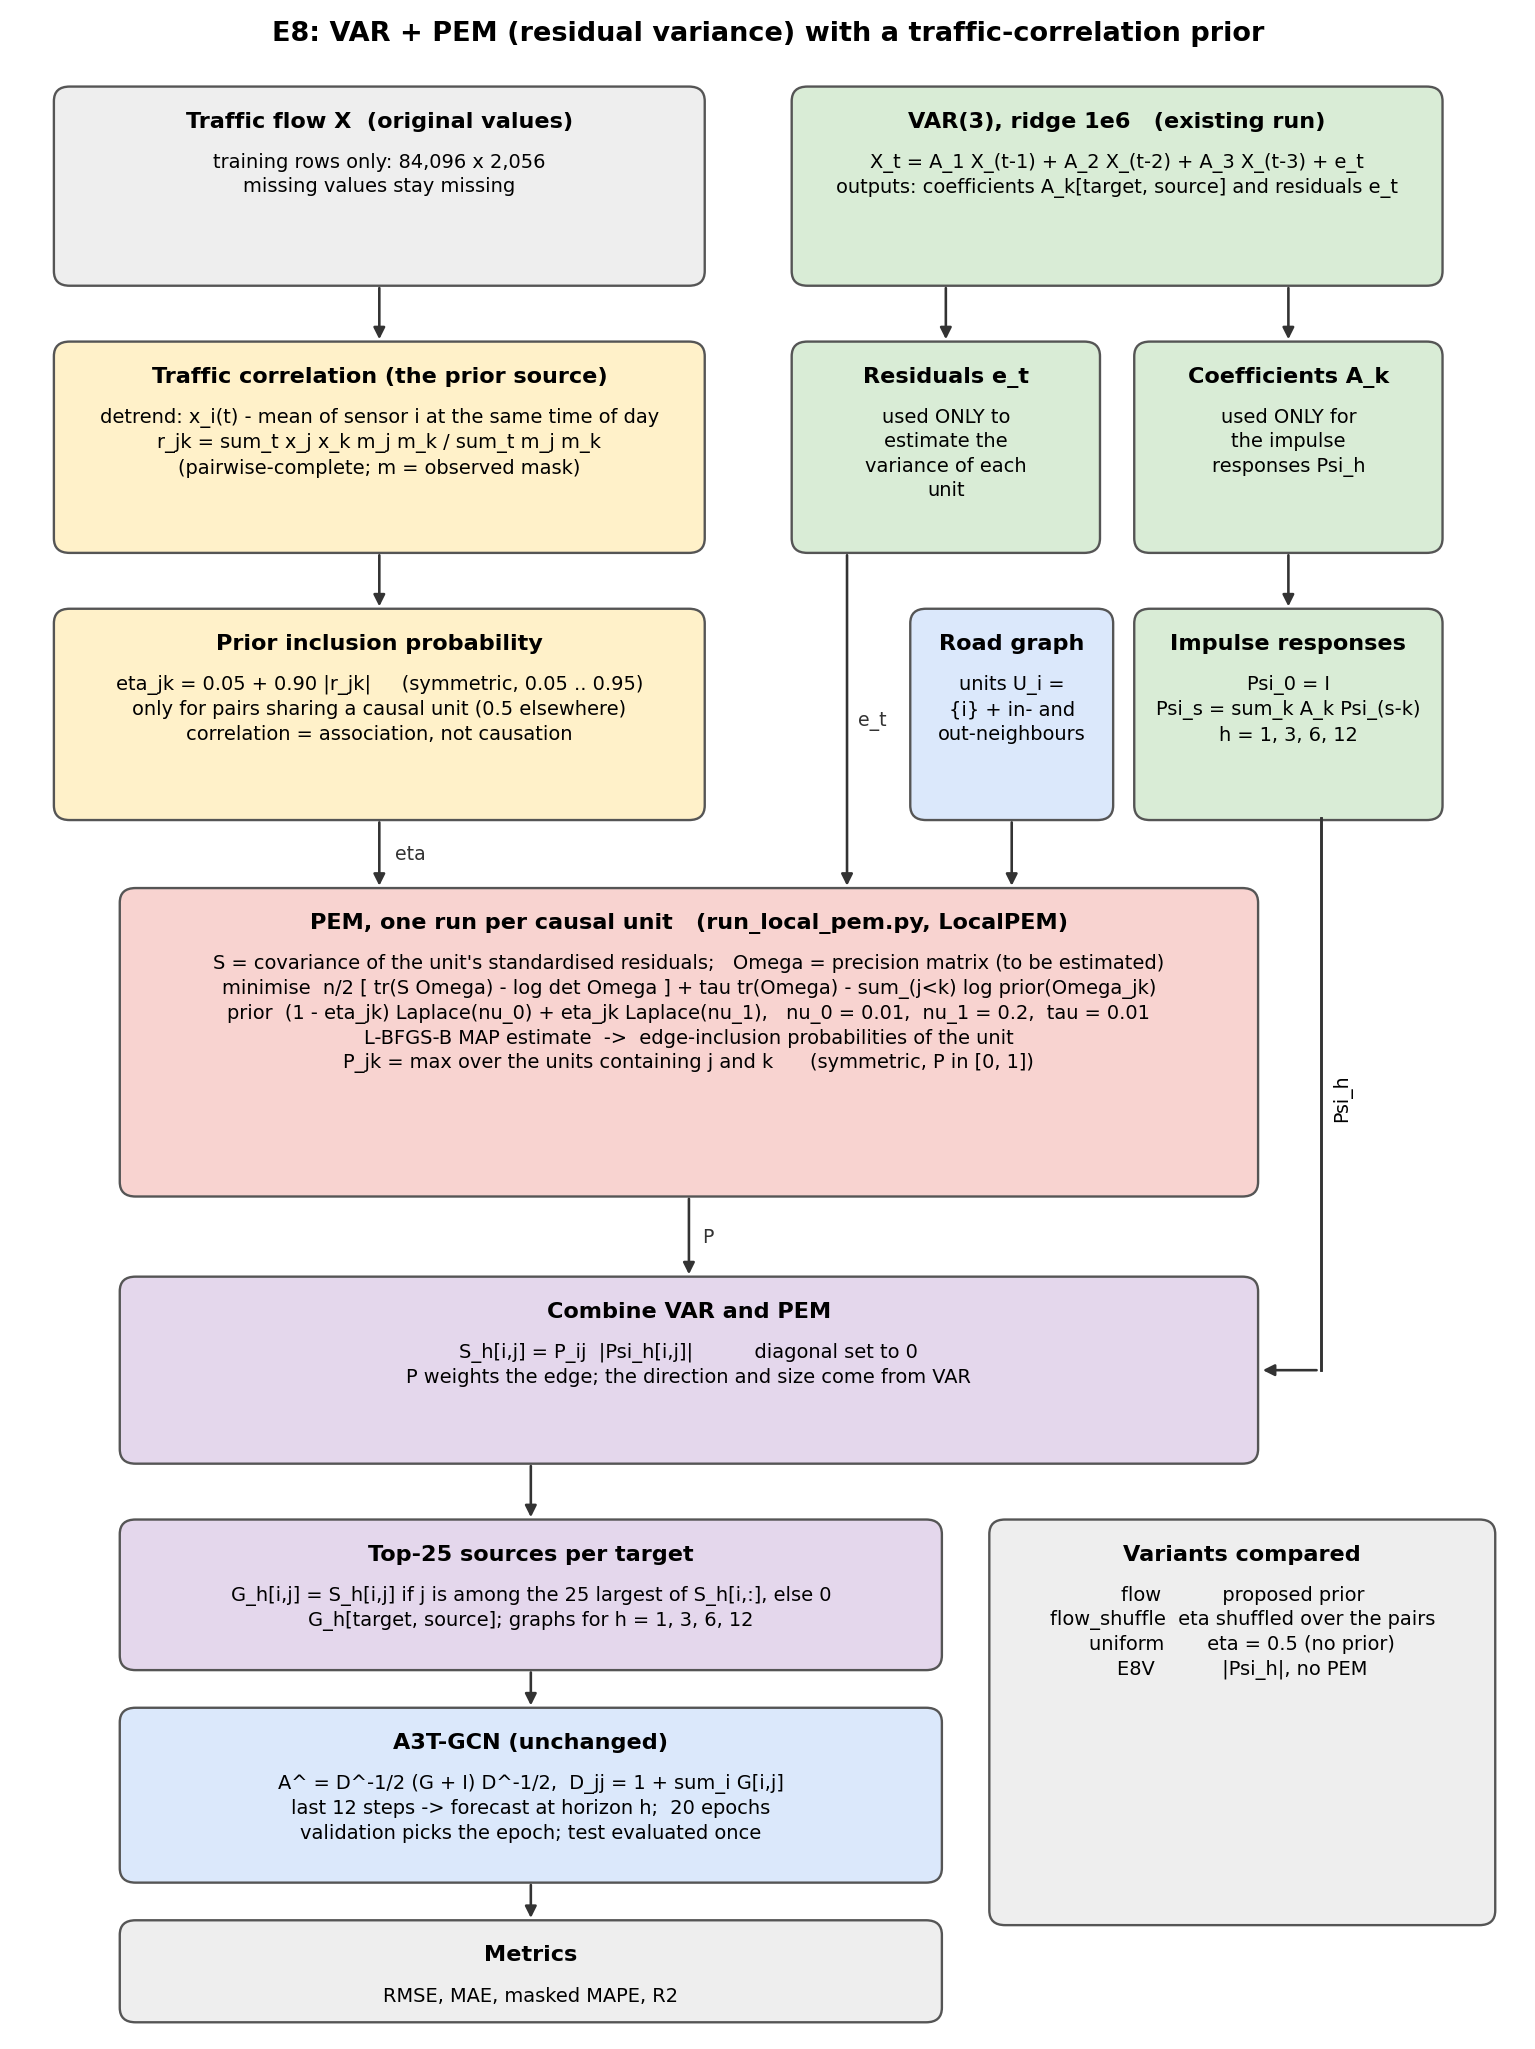
\includegraphics[width=0.98\textwidth]{e8_flowprior_pipeline.png}
\caption{The proposed construction. The correlation branch (left) produces the prior $\eta$; the VAR branch (right) produces residuals, used only for variance estimation, and coefficients, used only for impulse responses. PEM combines prior and residual structure into edge probabilities $P$, and the graph at horizon $h$ scores each edge by $P \odot |\Psi_h|$.}
\label{fig:pipeline}
\end{figure}

\section{Dataset and Experimental Platform}

\subsection{Dataset}
All experiments use the \ac{GBA} subset of the LargeST benchmark \citep{liu2023largest} for the year 2021: 105,120 five-minute intervals for 2,352 flow sensors, a directed road adjacency matrix, and sensor metadata. The raw files are never modified. Some sensors report nearly identical series, which makes covariance matrices singular and lets duplicated information masquerade as structure; two sensors are treated as copies when they agree on at least 90\% of commonly observed rows or correlate at 0.999 or above, judged on training rows only. Removing copies leaves 2,056 sensors, and this set is used by every stage. The data are split chronologically, 80\% / 10\% / 10\%: rows $[0, 84{,}096)$ for training, $[84{,}096, 94{,}608)$ for validation, and $[94{,}608, 105{,}120)$ for testing. Table~\ref{tab:data} collects the shared settings.

\begin{table}[htpb]
\small
\renewcommand{\arraystretch}{1.4}
\centering
\caption{Dataset and shared experimental settings.}
\label{tab:data}
\begin{tabular}{|p{6.5cm}|p{6.5cm}|}
\hline
Item & Value \\ \hline
Source & LargeST GBA, 2021, flow per 5 minutes \\ \hline
Rows $\times$ sensors (raw) & 105{,}120 $\times$ 2{,}352 \\ \hline
Sensors after duplicate removal & 2{,}056 \\ \hline
Chronological split & 80\% / 10\% / 10\% \\ \hline
Forecaster input / target & 12 steps / 1 step at horizon $h$ \\ \hline
Horizons $h$ & 1, 3, 6, 12 steps (5--60 minutes) \\ \hline
Sources kept per target ($K$) & 25 \\ \hline
Training & 20 epochs, Adam, learning rate 0.001, batch 8, gradient clip 5 \\ \hline
Model selection & lowest validation RMSE; test scored once \\ \hline
\end{tabular}
\end{table}

\subsection{Missing values and leakage control}
Roughly half of the test windows contain at least one missing reading. Discarding them wholesale would waste most of the test period, so gaps are filled, but only in the \emph{inputs} of the forecaster: short gaps by interpolation and longer gaps by a regression on neighbouring sensors fitted on training rows, with validation and test fills restricted to information available backward in time. Targets must be originally observed, and filled values are never scored. The statistical stages are stricter still: the VAR, the correlation prior, and PEM see only genuinely observed values, because a filled value is itself the output of a regression, and a dependence model fed such values would partly rediscover the filling procedure. Every estimator in the pipeline, including the scaler, the duplicate filter, the VAR, the prior, and PEM, is fitted on training rows alone.

\subsection{Platform}
The pipeline spans two environments. Graph construction and diagnostics run in a Python environment with NumPy and SciPy, on a local machine and on Kaggle CPU sessions; one full PEM pass over all 2,056 units costs roughly 23 CPU-hours and completes in just under six hours of wall time with four worker processes. Forecaster training runs on Kaggle GPU sessions (Tesla T4) in TensorFlow, at approximately 5.4 hours for a 20-epoch run. All heavy runs are committed notebook versions, so each result is tied to the exact code and inputs that produced it.

\section{The Correlation Branch: a Prior from the Traffic Itself}
\label{sec:prior}

Raw traffic series are correlated almost everywhere, because nearly every sensor rises in the morning and falls at night. The shared daily cycle must be removed before correlation can say anything about a specific pair. For sensor $i$, let $\mu_i(s)$ be the mean of its observed training values in time-of-day slot $s$ (there are 288 five-minute slots per day). The detrended series is
\begin{equation}
\tilde{x}_i(t) = x_i(t) - \mu_i\big(\mathrm{tod}(t)\big),
\label{eq:detrend}
\end{equation}
computed on training rows only. On this dataset the detrending matters a great deal: the median absolute correlation between road-adjacent sensors falls from 0.84 on raw series, a level so high that it cannot discriminate between pairs, to 0.44 after detrending.

For a pair $(j,k)$, the Pearson correlation $r_{jk}$ of $\tilde{x}_j$ and $\tilde{x}_k$ is computed over the rows where both sensors are observed, and set to zero when fewer than 1,000 common rows exist. The prior inclusion probability is then the affine map
\begin{equation}
\eta_{jk} \;=\; 0.05 + 0.90\,\lvert r_{jk}\rvert ,
\label{eq:eta}
\end{equation}
applied to every \emph{candidate pair}, meaning every pair that shares a causal unit in the sense of Section~\ref{sec:units}; all other pairs keep the neutral value $\eta_{jk}=0.5$, the diagonal is zero, and the matrix is symmetric. The bounds 0.05 and 0.95 keep the prior from becoming dogmatic in either direction: no pair is ruled out and none is ruled in before the data are consulted. Across the 138,548 candidate entries (69,274 unordered pairs) the realised prior has mean 0.51 and spans 0.050 to 0.946, so it is centred near neutrality while still spreading pairs apart.

It must be stressed that this prior encodes association, not causation. Two sensors may correlate because one influences the other, or because both respond to the same upstream demand. The construction therefore never lets the prior act alone: it only tilts the probability model, whose evidence comes from the conditional dependence structure of the residuals, and direction comes exclusively from the VAR branch.

\section{The VAR Branch: Directed Effects at Every Horizon}
\label{sec:var}

\subsection{Topology-aware estimation}
The flow vector $x(t) \in \mathbb{R}^{2056}$ is modelled as a lag-3 vector autoregression,
\begin{equation}
x(t) \;=\; \sum_{k=1}^{3} A_k\, x(t-k) \;+\; e(t),
\label{eq:var}
\end{equation}
estimated on training rows with a ridge penalty of $10^{6}$, both settings fixed in an earlier phase of the project by validation error. An unrestricted VAR on 2,056 series would estimate over twelve million coefficients per lag; instead, the support of each $A_k$ is restricted to road neighbours and the sensor itself, about 25 admissible sources per target, which is 1.2\% of all pairs. The restriction embodies the physical fact that five-minute influence travels along roads, and it is what makes the estimate stable. Rows with missing values are excluded rather than filled. The convention throughout is $A_k[i,j]$: the effect of source $j$ on target $i$ at lag $k$.

\subsection{Impulse responses}
A forecast $h$ steps ahead depends not only on direct lag-1 effects but on effects relayed through intermediate sensors. The impulse-response matrices of the fitted system capture exactly this accumulation:
\begin{equation}
\Psi_0 = I, \qquad
\Psi_s \;=\; \sum_{k=1}^{\min(s,3)} A_k\, \Psi_{s-k}, \qquad s = 1, 2, \ldots, h,
\label{eq:irf}
\end{equation}
so that $\Psi_h[i,j]$ is the total effect of a unit change at sensor $j$ on sensor $i$ after $h$ steps, summed over all paths. Note that $\Psi_1 = A_1$, while for $h>1$ the matrices fill in beyond the road support as effects propagate. Graphs are built for $h \in \{1, 3, 6, 12\}$, matching forecast horizons of 5 to 60 minutes. One property of the fitted system deserves record: its companion matrix has a largest eigenvalue of 1.05, marginally outside the stationary region, so $|\Psi_h|$ grows slowly with $h$ rather than decaying. Since each graph is normalised before use and horizons are never mixed, this affects the interpretation of weights across horizons rather than any single model, but it is reported here for completeness.

\subsection{Role of the residuals}
The residuals $e(t)$ of the VAR serve exactly one purpose in this framework: their variance structure, after standardisation, is the evidence on which the probability model operates. They are not used to build a separate residual graph, and no contemporaneous causal model (such as LiNGAM) is applied to them.

\section{The Probability Model}
\label{sec:pem}

\subsection{Causal units}
\label{sec:units}
Estimating one precision matrix over 2,056 variables is neither computationally feasible nor statistically advisable at this sample size. The estimation is therefore local: for each sensor $i$, the \emph{causal unit}
\begin{equation}
U_i \;=\; \{i\} \,\cup\, N_{\mathrm{in}}(i) \,\cup\, N_{\mathrm{out}}(i)
\label{eq:unit}
\end{equation}
collects the sensor and its road in- and out-neighbours, giving 2,056 overlapping units with typical sizes of twenty to seventy sensors. A pair of sensors is a \emph{candidate pair} when at least one unit contains both.

\subsection{Spike-and-slab precision estimation}
Within a unit $U$, the residuals of its sensors are standardised to unit variance, rows with any missing value are dropped, and the sample covariance $S_U$ is formed from the $n$ complete rows. PEM \citep{hwang2026pem} places on every off-diagonal entry of the precision matrix $\Omega$ a two-component mixture prior: a Laplace density $f_{\nu_0}$ sharply concentrated at zero (the spike, absent edge) and a wider Laplace density $f_{\nu_1}$ (the slab, present edge), mixed with the pair's prior weight $\eta_{jk}$ from Equation~\eqref{eq:eta}. The \ac{MAP} estimate solves
\begin{equation}
\min_{\Omega \succ 0}\;\;
\frac{n}{2}\Big[\operatorname{tr}(S_U\,\Omega) - \log\det\Omega\Big]
\;+\; \tau\operatorname{tr}\Omega
\;-\; \sum_{j<k}\log\!\Big[(1-\eta_{jk})\,f_{\nu_0}(\Omega_{jk}) + \eta_{jk}\,f_{\nu_1}(\Omega_{jk})\Big],
\label{eq:pemobj}
\end{equation}
with $\nu_0 = 0.01$, $\nu_1 = 0.2$, and $\tau = 0.01$, solved by L-BFGS-B with an SLSQP retry for the rare non-converged unit. At the optimum, the posterior probability that entry $(j,k)$ belongs to the slab is available in closed form,
\begin{equation}
P^{U}_{jk} \;=\;
\frac{\eta_{jk}\, f_{\nu_1}(\Omega_{jk})}
{\eta_{jk}\, f_{\nu_1}(\Omega_{jk}) + (1-\eta_{jk})\, f_{\nu_0}(\Omega_{jk})},
\label{eq:post}
\end{equation}
which rises with the magnitude of the estimated partial dependence $\Omega_{jk}$ and with the prior $\eta_{jk}$. Because units overlap, a pair may be estimated several times; the global probability is the maximum over the units containing the pair,
\begin{equation}
P_{jk} \;=\; \max_{U \,\supseteq\, \{j,k\}} P^{U}_{jk},
\label{eq:agg}
\end{equation}
a deliberately permissive rule, chosen because a dependence visible in any local context is worth retaining when the VAR magnitude will still have to confirm the edge. $P$ is symmetric with a zero diagonal, and no hard threshold is ever applied to it.

The scale parameters $(\nu_0, \nu_1)$ were revised from an earlier configuration after a sixty-unit pre-training check showed the original values saturating the probabilities; the revision used only the distribution of $P$, never any forecast result, and it is recorded here because the original values were set first.

\section{Combination, Selection, and the Forecaster}
\label{sec:combine}

The two branches meet in a single score per ordered pair and horizon:
\begin{equation}
S_h[i,j] \;=\; P_{ij}\,\bigl|\Psi_h[i,j]\bigr|, \qquad S_h[i,i] = 0 .
\label{eq:score}
\end{equation}
The division of labour is exact: direction and magnitude come from the VAR impulse response, and the symmetric probability $P$ scales each effect by the model's confidence that the pair is genuinely dependent. For each target $i$, the $K=25$ sources with the largest $S_h[i,j]$ are retained,
\begin{equation}
G_h[i,j] \;=\;
\begin{cases}
S_h[i,j] & \text{if } j \text{ is among the } K \text{ largest of row } i,\\[2pt]
0 & \text{otherwise},
\end{cases}
\label{eq:topk}
\end{equation}
which matches the in-degree of the road graph and keeps all variants comparable in density. The forecaster receives $G_h$ through the standard normalisation
\begin{equation}
\hat{A} \;=\; D^{-1/2}\,(G_h + I)\,D^{-1/2}, \qquad D_{jj} = 1 + \textstyle\sum_i G_h[i,j],
\label{eq:norm}
\end{equation}
and is otherwise untouched: A3T-GCN \citep{zhu2020a3tgcn} with a \ac{GRU} of 100 units and temporal attention, input length 12, trained for 20 epochs with Adam at learning rate 0.001, batch size 8, gradient clipping at 5, and L2 weight 0.0015. The learning rate halves after five epochs without validation improvement, the checkpoint with the lowest validation RMSE is restored, and the test set is evaluated once. A build-time check suite verifies, for every graph artefact, the orientation convention, the zero diagonal, the in-degree bound, symmetry of $P$, that every retained edge lies inside the support of $P$, and that no LiNGAM module or file is touched anywhere in the build.

\section{Controls and Reference Models}
\label{sec:controls}

A method with several ingredients needs controls that can fail it one ingredient at a time. Three internal variants are built under conditions identical to the proposed graph in every respect except the one under test.

\begin{table}[htpb]
\small
\renewcommand{\arraystretch}{1.4}
\centering
\caption{Internal variants and the question each answers. All use the same VAR, the same units, the same top-$K$ selection and the same forecaster.}
\label{tab:controls}
\begin{tabular}{|p{3.4cm}|p{4.6cm}|p{5.2cm}|}
\hline
Variant & Construction & Question answered \\ \hline
Flow prior (proposed) & $\eta$ from Eq.~\eqref{eq:eta} & -- \\ \hline
Uniform prior & $\eta_{jk} = 0.5$ everywhere & Does any prior information help over none? \\ \hline
Shuffled prior & flow-prior values permuted among candidate pairs (fixed seed) & Is it the information, or merely the value distribution? \\ \hline
VAR-only (no PEM) & $S_h = |\Psi_h|$ & Does probabilistic weighting help at all? \\ \hline
\end{tabular}
\end{table}

The logic of Table~\ref{tab:controls} is worth spelling out. If the proposed graph outperforms the uniform prior but not the shuffled prior, the benefit comes from the shape of the prior distribution, not from assigning the right values to the right pairs. If it outperforms neither, the prior is uninformative in effect. And if none of the three outperforms the VAR-only variant, then PEM as a whole, prior included, contributes nothing measurable to forecast accuracy; the criterion adopted in advance is that PEM is considered useful only if the proposed graph beats the VAR-only ablation. Figure~\ref{fig:e8v} shows the VAR-only construction.

External references complete the design: the unweighted road graph, the VAR-weighted road graph (the matrix $\sum_k |A_k|$ on road support), a graph-free model in which the graph operator is the identity so that each sensor is forecast from its own history by the \ac{GRU} and attention alone, and the historical average, which predicts each sensor's weekday-and-slot mean.

\begin{figure}[htpb]
\centering
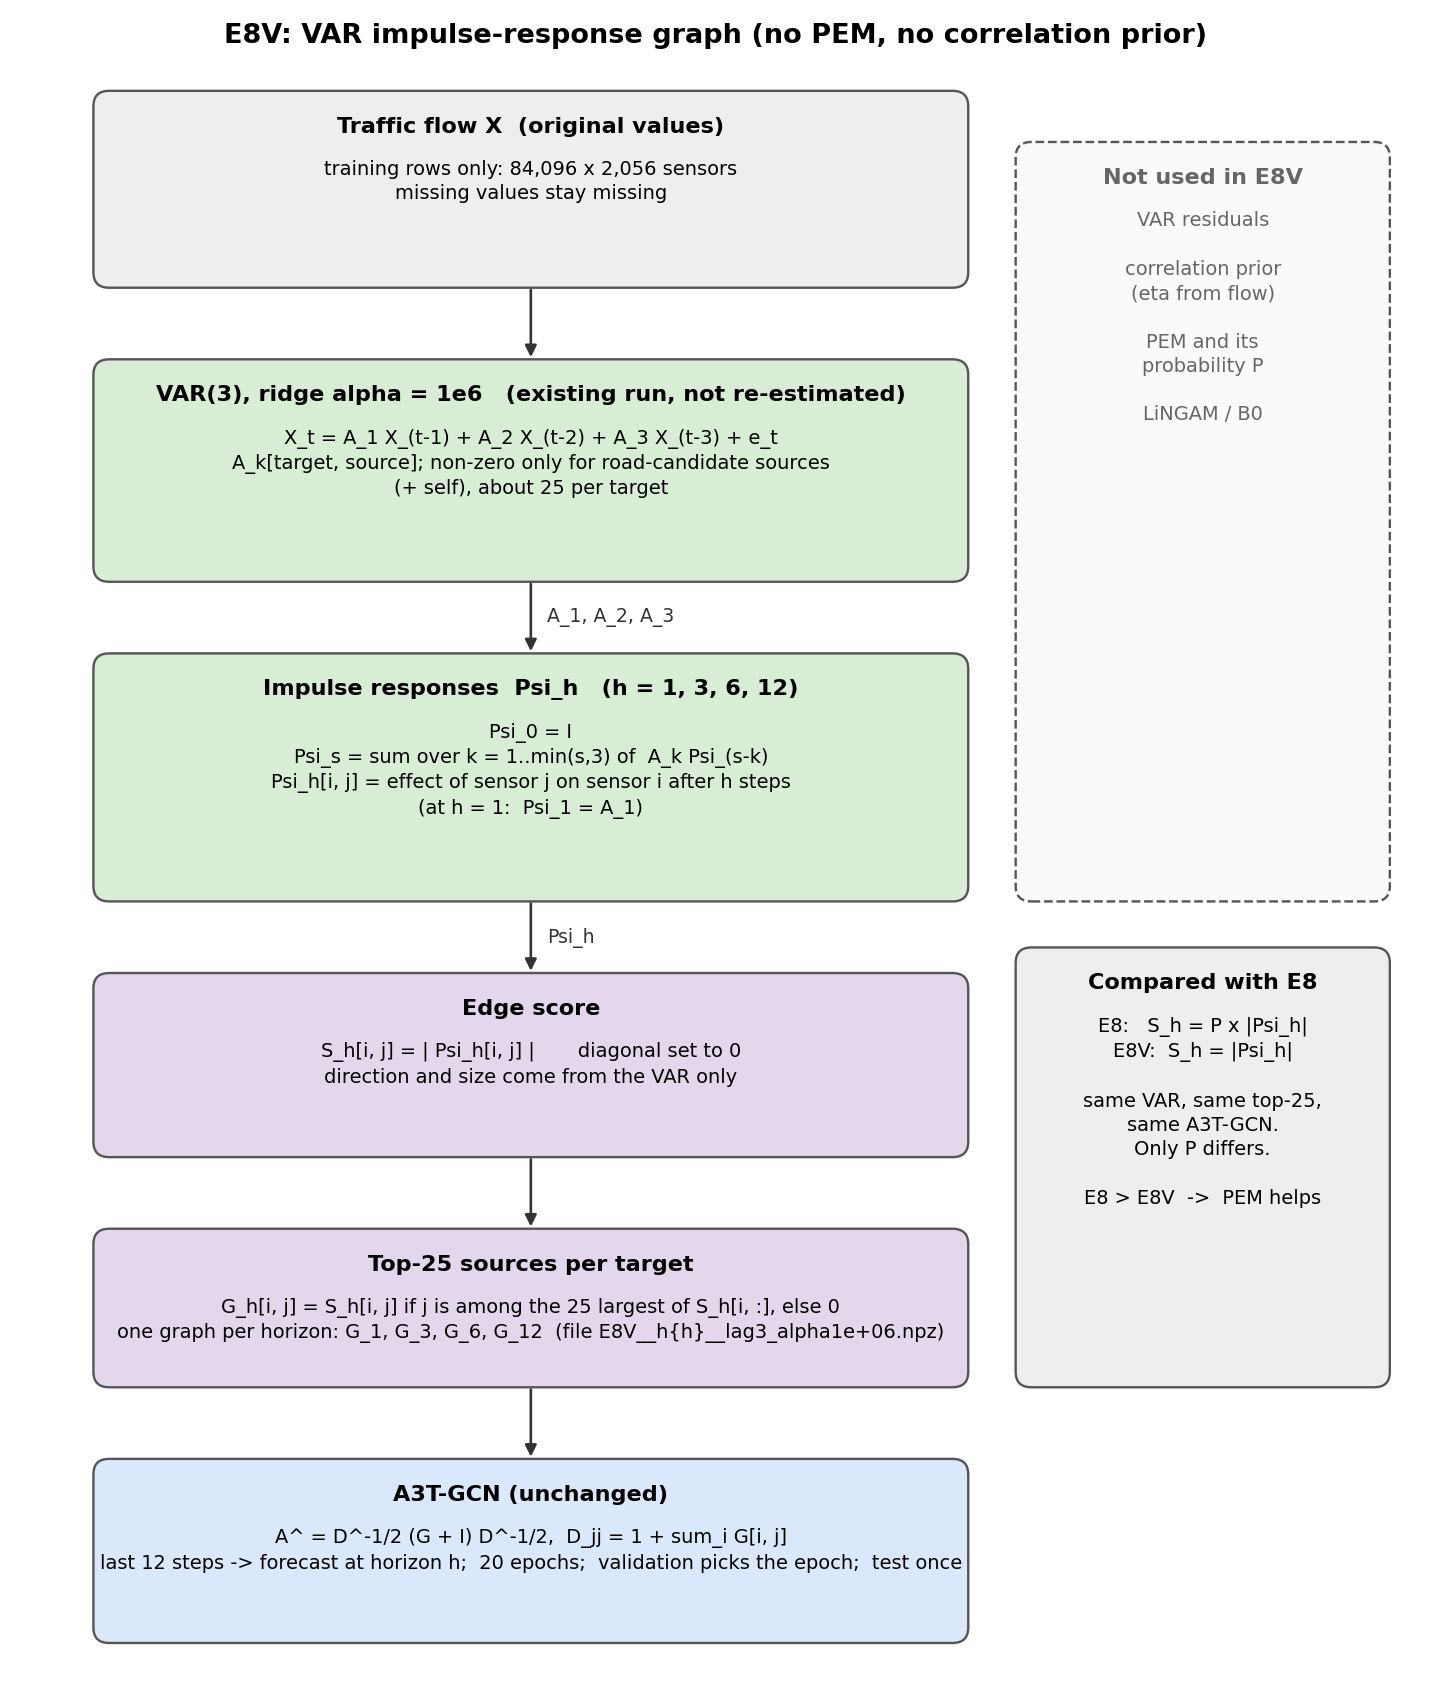
\includegraphics[width=0.9\textwidth]{e8v_pipeline.png}
\caption{The VAR-only ablation. The correlation prior, the residuals and PEM are removed; the edge score is $|\Psi_h|$ alone. Comparing this variant with the proposed graph isolates the contribution of the probability model.}
\label{fig:e8v}
\end{figure}

\section{Evaluation Protocol}
Metrics are \ac{RMSE}, \ac{MAE}, masked \ac{MAPE} (computed over targets of at least 10 vehicles to avoid division by near-zero counts), and $R^2$, in vehicles per five minutes, pooled over test windows and sensors. Every graph variant trains with the identical frozen settings of Table~\ref{tab:data}; only the graph file changes between runs, which the training harness verifies mechanically by checking the graph's recorded horizon, sensor list and training split against the run configuration. Seed 42 is the primary seed, with seeds 7 and 123 reserved for repetition, because earlier reference runs showed that the seed alone can move the test RMSE of this forecaster by more than one vehicle per five minutes; a difference between two graphs is treated as meaningful only when it exceeds this spread.

%------------------------------------------------------------------------------------------------%
% REFERENCES FOR PART 1
% These pages exist only so that the citations in Chapters 1-3 resolve while this part is compiled.
% When merging the PDFs, DROP every page of Part 1 that follows the last page of Chapter 3.
% The complete reference list is in Part 2.
\begin{singlespace}
  \bibliography{thesis_refer}
\end{singlespace}
% Pull the contents / figure / table entries of Part 2 into the lists of THIS part (optional, see README).
% Harmless when the files are missing.
\addtocontents{toc}{\protect\InputIfFileExists{thesis_part2.toc}{}{}}
\addtocontents{lof}{\protect\InputIfFileExists{thesis_part2.lof}{}{}}
\addtocontents{lot}{\protect\InputIfFileExists{thesis_part2.lot}{}{}}
\end{document}
